\documentclass[aps,pra,superscriptaddress,twocolumn]{revtex4-1}

\usepackage{graphicx}
\usepackage{amsmath}
\usepackage{amssymb}
\usepackage{hyperref}
\usepackage[utf8]{inputenc}
\usepackage{mathtools}
\usepackage[english]{babel}
\usepackage{bbm}
\hypersetup{colorlinks=true, linkcolor=blue, citecolor=blue, urlcolor=blue}
\usepackage{xcolor}
\usepackage{braket}

%===Newcommands============================
\DeclareMathOperator{\sgn}{sgn}
\newcommand{\ie}{i.\,e.,\ }
\newcommand{\Ie}{I.\,e.\,,\ }
\newcommand{\eg}{e.\,g.,\ }
\newcommand{\Eg}{E.\,g.\,,\ }
\newcommand{\cf}{cf.\ }
%
\newcommand{\re}{\mathrm{Re}}
\newcommand{\im}{\mathrm{Im}}
\newcommand{\abs}[1]{|#1|}
\newcommand{\ii}{\mathrm{i}}
\newcommand{\ee}{\mathrm{e}}
\newcommand{\proj}[1]{|#1\rangle\langle #1|}
\newcommand{\Tr}{\operatorname{Tr}}
\newcommand{\rr}{\mathbf{r}}
\newcommand{\pp}{\mathbf{p}}
\newcommand{\kk}{\mathbf{k}}
%
\newcommand{\cc}{\text{c.c.}}
\newcommand{\fref}[1]{\text{Fig.}~\ref{#1}}
\newcommand{\ffref}[1]{\text{Figs.}~\ref{#1}}
\newcommand{\eref}[1]{\text{Eq.}~\eqref{#1}}
\newcommand{\eeref}[1]{\text{Eqs.}~\eqref{#1}}
%
\newcommand{\commentSB}[1]{\texttt{\color{blue}[#1]}}
\newcommand{\commentSO}[1]{\texttt{\color{orange}[#1]}}
\newcommand{\commentTP}[1]{\texttt{\color{green}[#1]}}
\newcommand{\commentOR}[1]{\texttt{\color{yellow}[#1]}}
\newcommand{\commentSY}[1]{\texttt{\color{red}[#1]}}

%==============================================================================================
\begin{document}
\title{Optimized geometries for optical lattices}
\author{A}
% \email{}
\affiliation{Department of Physics, Harvard University, Cambridge, Massachusetts 02138, USA}
\author{B}
% \email{}
\affiliation{Department of Physics, Harvard University, Cambridge, Massachusetts 02138, USA}
\author{C}
% \email{}
\affiliation{Department of Physics, Harvard University, Cambridge, Massachusetts 02138, USA}

\begin{abstract}

This is the abstract. 

\end{abstract}

\maketitle

%==============================================================================================
\section{Introduction}

% This is the introduction, see~\fref{fig:setup}.
% % \commentSB{not sure about this statement}

% \begin{equation}
% H = p^2
% \label{eqn:Hamiltonian}
% \end{equation}

\begin{figure}
\centering
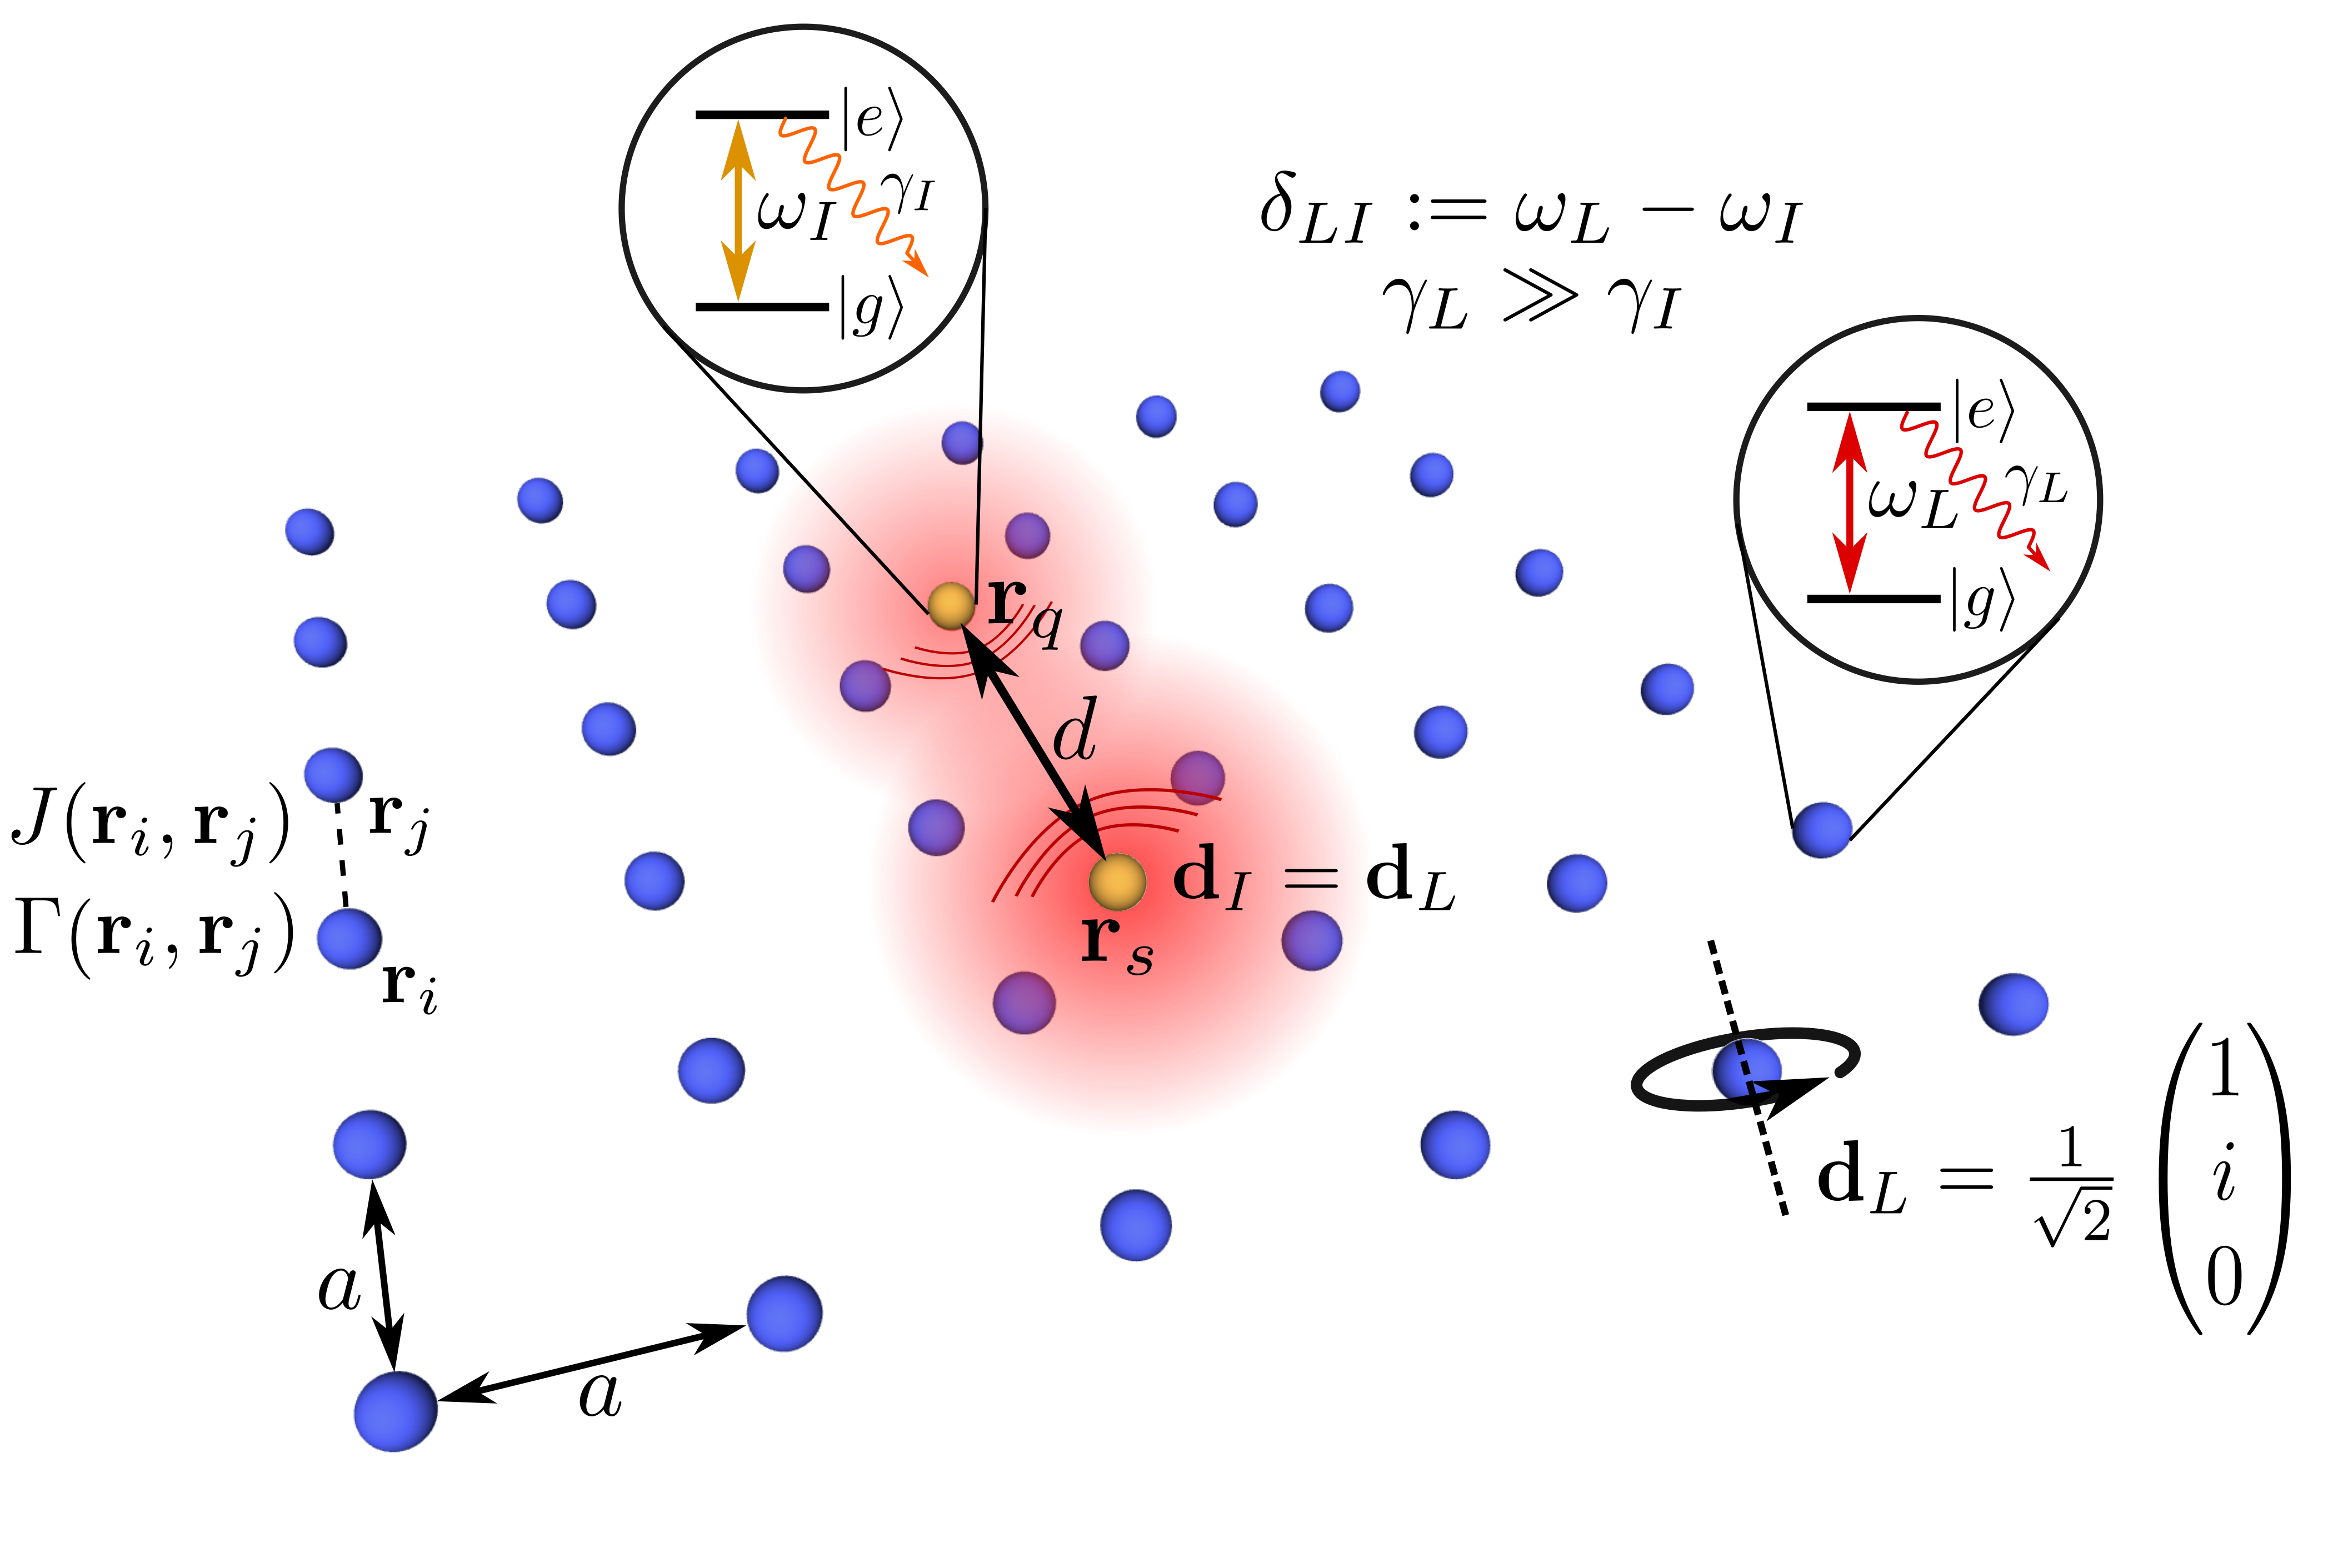
\includegraphics[width=0.4\textwidth]{figures/setup_2.png} 
\caption{•}
\label{fig:setup}
\end{figure}

% We see in~\eeref{eqn:Hamiltonian} and~\fref{fig:setup},~\eg test~\cite{kramer_quantumopticsjl_2018}

%==============================================================================================
\section{Model}
\commentSO{arb. geometry, Green's Tensor, Couplings, Polarizations -> Distance dependence, Hamiltonian, Self-energy, Ref. to Taylor's work}

We consider two-dimensional sub-wavelength lattices of quantum emitters which interact via resonant dipole-dipole interactions. The emitters are assumed to be two-level stems with a ground state $\ket{g}$ and an excited state $\ket{e}$ with a trasition frequency $\omega_L = c k_L$. Where $k_L = 2\pi/\lambda_L$ denotes the related wavenumber with the resonance wavelegth $\lambda_L$. Pairwise resonant dipole-dipole interactions among emitters result in collective couplings and decay rates between emitters $i$ and $j$ at positions $\rr_i$ and $\rr_j$, which are given as

% We consider each type of Bravais lattice.

% Where possible, we set the characteristic inter-atomic spacing to be a factor of 0.2 of the lattice's resonant wavelength 

% \commentTP{"We consider a subwavelength lattice, with a distance between the atoms that is smaller than their resonant wavelength"}

\commentTP{Put J and Gamma before the Green's tensor, e.g. "We consider }



% \commentSB{Is this choice of 0.2 based off of Taylor's findings? In that case, cite her here.}
% \commentSB{Also, for something like the triangular plot, shouldn't we choose $a$ such that there is constant area?} 


The Green's tensor is 

% \begin{equation}

% \end{equation}

\begin{equation} \resizebox{1.0\hsize}{!}{
    $ \textbf{G}(\textbf{r},\omega) = \begin{pmatrix}
        \frac{e^{i\omega r}}{4\pi r} \left[ \left( 1 + \frac{i}{\omega r} - \frac{1}{\omega^2 r^2} \right) - \left( 1 + \frac{3i}{\omega r} - \frac{3}{\omega^2 r^2} \right) \frac{r_x r_x}{r^2} \right] - \frac{\delta(\textbf{r})}{3\omega^2}
        & -\frac{e^{i\omega r}}{4\pi r} \left( 1 + \frac{3i}{\omega r} - \frac{3}{\omega^2 r^2} \right) \frac{r_x r_y}{r^2}
        & -\frac{e^{i\omega r}}{4\pi r}  \left( 1 + \frac{3i}{\omega r} - \frac{3}{\omega^2 r^2} \right) \frac{r_x r_z}{r^2}  \\
        - \frac{e^{i\omega r}}{4\pi r} \left( 1 + \frac{3i}{\omega r} - \frac{3}{\omega^2 r^2} \right) \frac{r_y r_x}{r^2}  
        & \frac{e^{i\omega r}}{4\pi r} \left[ \left( 1 + \frac{i}{\omega r} - \frac{1}{\omega^2 r^2} \right) - \left( 1 + \frac{3i}{\omega r} - \frac{3}{\omega^2 r^2} \right) \frac{r_y r_y}{r^2} \right] - \frac{\delta(\textbf{r})}{3\omega^2} 
        & - \frac{e^{i\omega r}}{4\pi r} \left( 1 + \frac{3i}{\omega r} - \frac{3}{\omega^2 r^2} \right) \frac{r_y r_z}{r^2} \\
        - \frac{e^{i\omega r}}{4\pi r} \left( 1 + \frac{3i}{\omega r} - \frac{3}{\omega^2 r^2} \right) \frac{r_z r_x}{r^2} 
        & - \frac{e^{i\omega r}}{4\pi r} \left( 1 + \frac{3i}{\omega r} - \frac{3}{\omega^2 r^2} \right) \frac{r_z r_y}{r^2} 
        & \frac{e^{i\omega r}}{4\pi r} \left[ \left( 1 + \frac{i}{\omega r} - \frac{1}{\omega^2 r^2} \right) - \left( 1 + \frac{3i}{\omega r} - \frac{3}{\omega^2 r^2} \right) \frac{r_z r_z}{r^2} \right] - \frac{\delta(\textbf{r})}{3\omega^2}
    \end{pmatrix} $
    \label{eqn:green}
    }\end{equation}
    \commentSB{This can't be put here; the sizing is all wrong.}

    \commentTP{From here on to the end of this section, remember to tell the reader what every one of these variables means. This is a good way of introducing things like the polarization, etc.}

    \commentTP{Put Green's tensor as Taylor defines it}

    Couplings between dipoles are governed coherent and incoherent terms, respectively, 
    \commentSB{This idea of "coherent" and "incoherent" terms is taken from Taylor's paper, and deserves more explanation.}
    \commentSB{Also, the way in which these two terms fit into the Hamiltonian should be made clear.}

    \commentTP{Collective couplings/frequency shifts and collective dissipations}

    $$
        J_{ij} = -\frac{3\pi \sqrt{\gamma_i \gamma_j}}{\omega_L} {\hat{d}^\dagger}_i \cdot \textbf{Re} [\textbf{G}(\textbf{r}_{ij}, \omega_L)] \cdot \hat{d}_j 
        \label{eqn:J}
    $$
    $$
        \Gamma_{ij} = \frac{6\pi \sqrt{\gamma_i \gamma_j}}{\omega_L} {\hat{d}^\dagger}_i \cdot \textbf{Im} [\textbf{G}(\textbf{r}_{ij},\omega_L)] \cdot \hat{d}_j 
        \label{eqn:Gamma}
    $$

    \commentTP{Put every type of equation you can think of}

    We place one or two lattice impurities with transition frequency $\omega_I \approx \omega_L$. 

    % \commentSB{It may be worth enumerating these equations with "a" and "b" instead of separate numbers}
    % \commentSB{Also, as a note to myself, watch out for vectors that need to be changed to bold rather than being under arrows}

    Both the lattice dipoles and impurity diples are given circular polarizations, so that their dynamics are independent of their relative orientations.
    \begin{equation} 
        \hat{d}_L = \hat{d}_I = \frac{1}{\sqrt{2}} \begin{pmatrix}
        1 \\ i \\ 0
        \end{pmatrix} 
        \label{eqn:polarization}
    \end{equation}
    As a result, the strength of couplings depends purely on the relative distances $r_{ij}$ between pairs of dipoles. 

    \commentSB{Put the figures of J over r, and Gamma over r here. Put this possibly alongside the setup picture.}

    \commentSB{Then, at some point here or later, explain the role of the detuning $\delta_{LI}$}

    % For further information, see~\cite{patti_controlling_2021}.

    % \commentSB{This is a very inelegant way of referencing Taylor's work on my part. This citation should probably go earlier, perhaps as soon as J and Gamma are mentioned.}

    The the most general form of the Hamiltonian is then
    \begin{equation}
        H = 
        \begin{pmatrix}
            -\frac{i \gamma_L}{2} - \frac{\delta_{LI}}{2} & J(r_{12}) - \frac{i \Gamma(r_{12})}{2} & \cdots \\
            J(r_{21}) - \frac{i \Gamma(r_{21})}{2} & -\frac{i \gamma_L}{2} - \frac{\delta_{LI}}{2} & & \\
            \vdots & & \ddots

        \end{pmatrix}
    \end{equation}
    \commentTP{Write Hamiltonian in terms of sigmas and s. Put this lattice definition in later sections.}

    % \commentSB{I haven't written out this Hamiltonian in full, because my first question is whether such a general Hamiltonian is even worth writing out. Will it be obvious to the reader?}

    \commentSB{Now, for the self-energy calculation, since there is a certain amount of difference between this calcualation for the single impurity case and the double impurity case, should these calculations be written out individually, in the single-impurity and double-impurity sections - Yes put in individual sections}



%==============================================================================================
\section{Single impurity case}
\commentSO{Define lattices, define distances related to lattices, $\Gamma_\mathrm{eff}$, constant area}

\commentSB{Put the self-energy calculation here, along with the Gamma-eff calculation? Because I don't think there's anything more to say here. Any details about the geometries need to be left to the specific sections directly below here.}
\commentTP{Draw a diagram of the four parts of the Hamiltonian to set up the self-energy calculation.}


In order to reasonably compare lattices of differing geometries, we ensure whenever possible that all plaquettes possess the same area.
% , because...
% \commentSB{Does this argument rely on a momentum-space view of things? In any case, make this constant area argument rigorous}

\subsection{Square vs. triangular}

Consider a finite square lattice, with an inter-atomic spacing of $a = 0.2$, defined as a function of \commentSB{that characteristic wavelength}. 

Compare this to a triangular lattice with the same inter-atomic spacing. 
\commentSB{see earlier point about how we should really use constant area}

\commentTP{Put a figure that just shows a single plaquette for each of our two cases here, with dots going off in 4 and 3 directions respectively}

%=================
\subsubsection{Interstitial}
\commentSO{Interstitial which imposes one more length scale -> refer to analytics, numerics -> impurity position}
Now, consider an impurity atom placed within a plaquette. For the square case, we implemented this arrangement using a $4\times 4$ lattice, so that the impurity was centered within the lattice. 

\commentSB{Put a small diagram here? You can illustrate the length scales here as well}

Likewise, for the triangular case, we placed the impurity at the center of a \commentSB{12 atom?} lattice, with the following arrangement. 

\commentSB{diagram?}

By placing the impurity at the center of a plaquette, only one additional length scale is introduced. 
% Hence, the coupling as a function of inter-atomic spacing is \commentSB{fairly constant, looking at the analytics?} 

% \commentSB{J and Gamma diagrams}

% \commentSB{Should we vary inter-atomic spacing?}

After attempting to place the impurity off-center, 

\commentTP{Have a plot of Gamma over delta, to justify how we choose an "optimum" delta}

\commentSB{numerics plaquette plots}

it is clear that the point at which the impurity atom experiences minimal decay is at the center of the plaquette. 

\commentSB{plaquette lineplots showing minimal Gamma}

This point also possesses the highest symmetry, suggesting that additional symmetries lead to slower decay rates. This hypothesis is supported by the behavior of the coupling constants for various positions of the impurity away from the center 

\commentSB{a diagram of this description, which has not been made yet. Or perhaps two diagrams, one moving from the center to a lattice point, and another moving from the center to the midpoint between two lattice points. Actually, four diagrams, because these two should be made for both the square and triangular cases}


%=================
\subsubsection{Substitution}
\commentSO{Does NOT(!) impose another length scale as long as it is not away from the center -> refer to analytics, -> always at band edge, numerics -> impurity position}

Now, considering substituting a lattice atom for an impurity, so that, in effect, the impurity takes up a vacancy in the lattice. For the square lattice, we used this $5 \times 5$ geometry for our analysis:

\commentSB{diagram}

and for the triangular lattice, we used this geometry

\commentSB{probably an 18 atom lattice?}

Performing this substitution on the lattice introduces no additional length scales, as long as the impurity is placed at the center of the vacancy. If it is placed off-center, the best possible values of $\Gamma_\text{eff}$ are 

\commentSB{plaquette plots from numerics}

Once again, the point with the highest symmetry experience  minimal decay rates

\commentSB{plaquette lineplots showing minimal Gamma}

\commentSB{Maybe include another analytic plot showing how symmetry changes coupling constants? Just do this for square lattice.}

%==============================================================================================
\subsection{Monoclinic vs. rectangular lattice}
\commentSO{similar arguments}

Now, consider the Bravais lattices defined by variable paramters. 

In particular, consider a monoclinic lattice defined by $\theta$, such that at $\theta = \frac{\pi}{2}$ we recover the square lattice case with an inter-atomic spacing of $0.2$. By maintaining a constant vertical distance between the layers of the lattice, we ensure that the area of the plaquettes remains constant over the range $ 0 < \theta \leq \frac{\pi}{2}$. 

\commentSB{diagram of this geometry}

%=================
\subsubsection{Interstitial}


%=================
\subsubsection{Substitution}

%=================
\subsubsection{Varying scaling factors}
\commentSO{justify why we use interstitial in the following}

%==============================================================================================
\section{Two impurity case}
\commentSO{Q-factor, analyze different lattices -> discuss the most important figures, constant distance}

%=================
\subsection{Monoclinic lattice}


%=================
\subsection{Rectangular lattice}


%==============================================================================================
\section{Conclusions and Outlook}\label{sec:conclusion}

These are the Conclusions.\\[2ex]

\emph{Acknowledgments.} We would like to thank \commentSO{add people}. This work was supported by \commentSO{add funding sources}

The numerical simulations were performed with the open-source framework \texttt{QuantumOptics.jl}~\cite{kramer_quantumopticsjl_2018}.


\bibliographystyle{apsrev4-1-title}
\bibliography{references_optimized_geometries}

\end{document}

